\chapter{Teorii și tehnologii utilizate}

În acest capitol sunt prezentate în primul rând tehnologiile utilizate în implementarea aplicației. În cea de a doua parte este evidențiat în mare parte particularități ale algoritmicii utilizate în determinarea unei alocări optime specifice problemei, în alte cuvinte algoritmul de \textit{stable matching} (\textit{stable marriage}).

\section{Angular}
\begin{figure}[H]
	
\includegraphics[width=0.3\textwidth, left]{Angular-logo.png}
%	\caption{\url{https://www.vectorlogo.zone/logos/angular/angular-ar21.png}}
\end{figure}

\textbf{Angular} este un framework de JavaScript scris în TypeScript și menținut de Google. Framework-ul a fost dezvoltat în principal pentru crearea aplicațiilor web \textit{single-page}, într-o manieră ce ușurează mentenanța și dezvoltarea ulterioară.

\subsection{Scurt istoric}
În 2010, Miško Hevery, un angajat la Google la acel timp, a lansat un proiect cu numele \textit{AngularJS} care a fost apreciat în mare măsură de comunitate. Între anii 2014-2015 a avut loc o reîmprospăatare majoră a framework-ului însemnând de fapt o rescriere majoră a acestuia. Noua versiune avea să fie numită simplu Angular. Au urmat câțiva ani de tranziție deoarece multe proiecte deja în producție erau utilizau AngularJS și  trebuiau refactorizate. În acest moment, Angular este cel mai folosit framework de front-end, în specialde dezvoltatorii de la Google și de către start-up-uri. Exemple de companii recunoscute ce folosesc Angular sunt Microsoft, Gmail, PayPal, Forbes.

\begin{figure}[H]
	\centering
	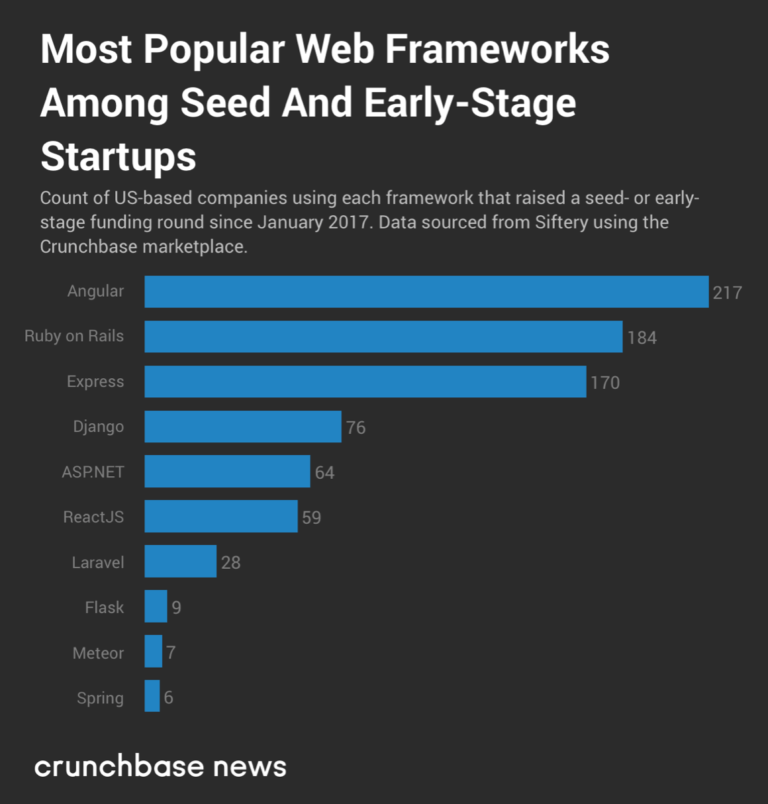
\includegraphics[width=0.8\textwidth]{Angular-crunchbase-newspng.png}
	\caption{\url{https://www.moveoapps.com/blog/how-to-use-angular-development/}}
\end{figure}

\subsection{Particularități}
Motivul alegerii Angular pe partea de front-end este reprezentat de o serie de caracteristici.

Un astfel de motiv este \textit{arhitectura bazată pe componenta}, fiind astfel o formă de programare orientată pe obiect. Utilizatorul crează în mod uzual clase corespunzătoare componentelor ce conțin și un șablon HTML (\textit{eng.} HTML template). Pentru simplificare, Angular oferă și opțiunea de "injectare" a serviciilor \textit{custom} sau \textit{in-built} într-o componentă ce utilizează aceste funcționalități. În acest fel, utilizatorul poate reutiliza, înlocui, modifica componente în diverse locuri, obținâându-se astfel un UI (User Interface) modularizat.

Un alt motiv este modul de încărcare a paginii web. Angular folosește \textit{lazy loading} ce permite încărcarea instantanee a website-urilor, prin afișarea doar a componentelor cerute și necesare utilizatorului, în timp ce celelalte sunt pregătite în fundal pentru alte eventualități.

\textit{Dependency injection} reprezintă un al treilea motiv, un design pattern ce permite împărțirea lucrului între diferite servicii, distribuind în mod eficient sarcinile. Prin inițializarea dependențelor, Angular reușește să reducă în mod considerabil codul de tip \textit{boilerplate} (fragmente similare de cod des utilizat între care există mici diferențe) și să extindă mai ușor o astfel de aplicație.

Framework-ul are trei tipuri de \textit{dependency injections}:
\begin{enumerate}
	\item Constructor injection
	\item Setter injection
	\item Interface injection
\end{enumerate}

Din punct de vedere al arhitecturii, Angular este în totalitate un framework MVC (model-view-controller), după cum se observă în figura următoare.

\begin{figure}[H]
	\centering
	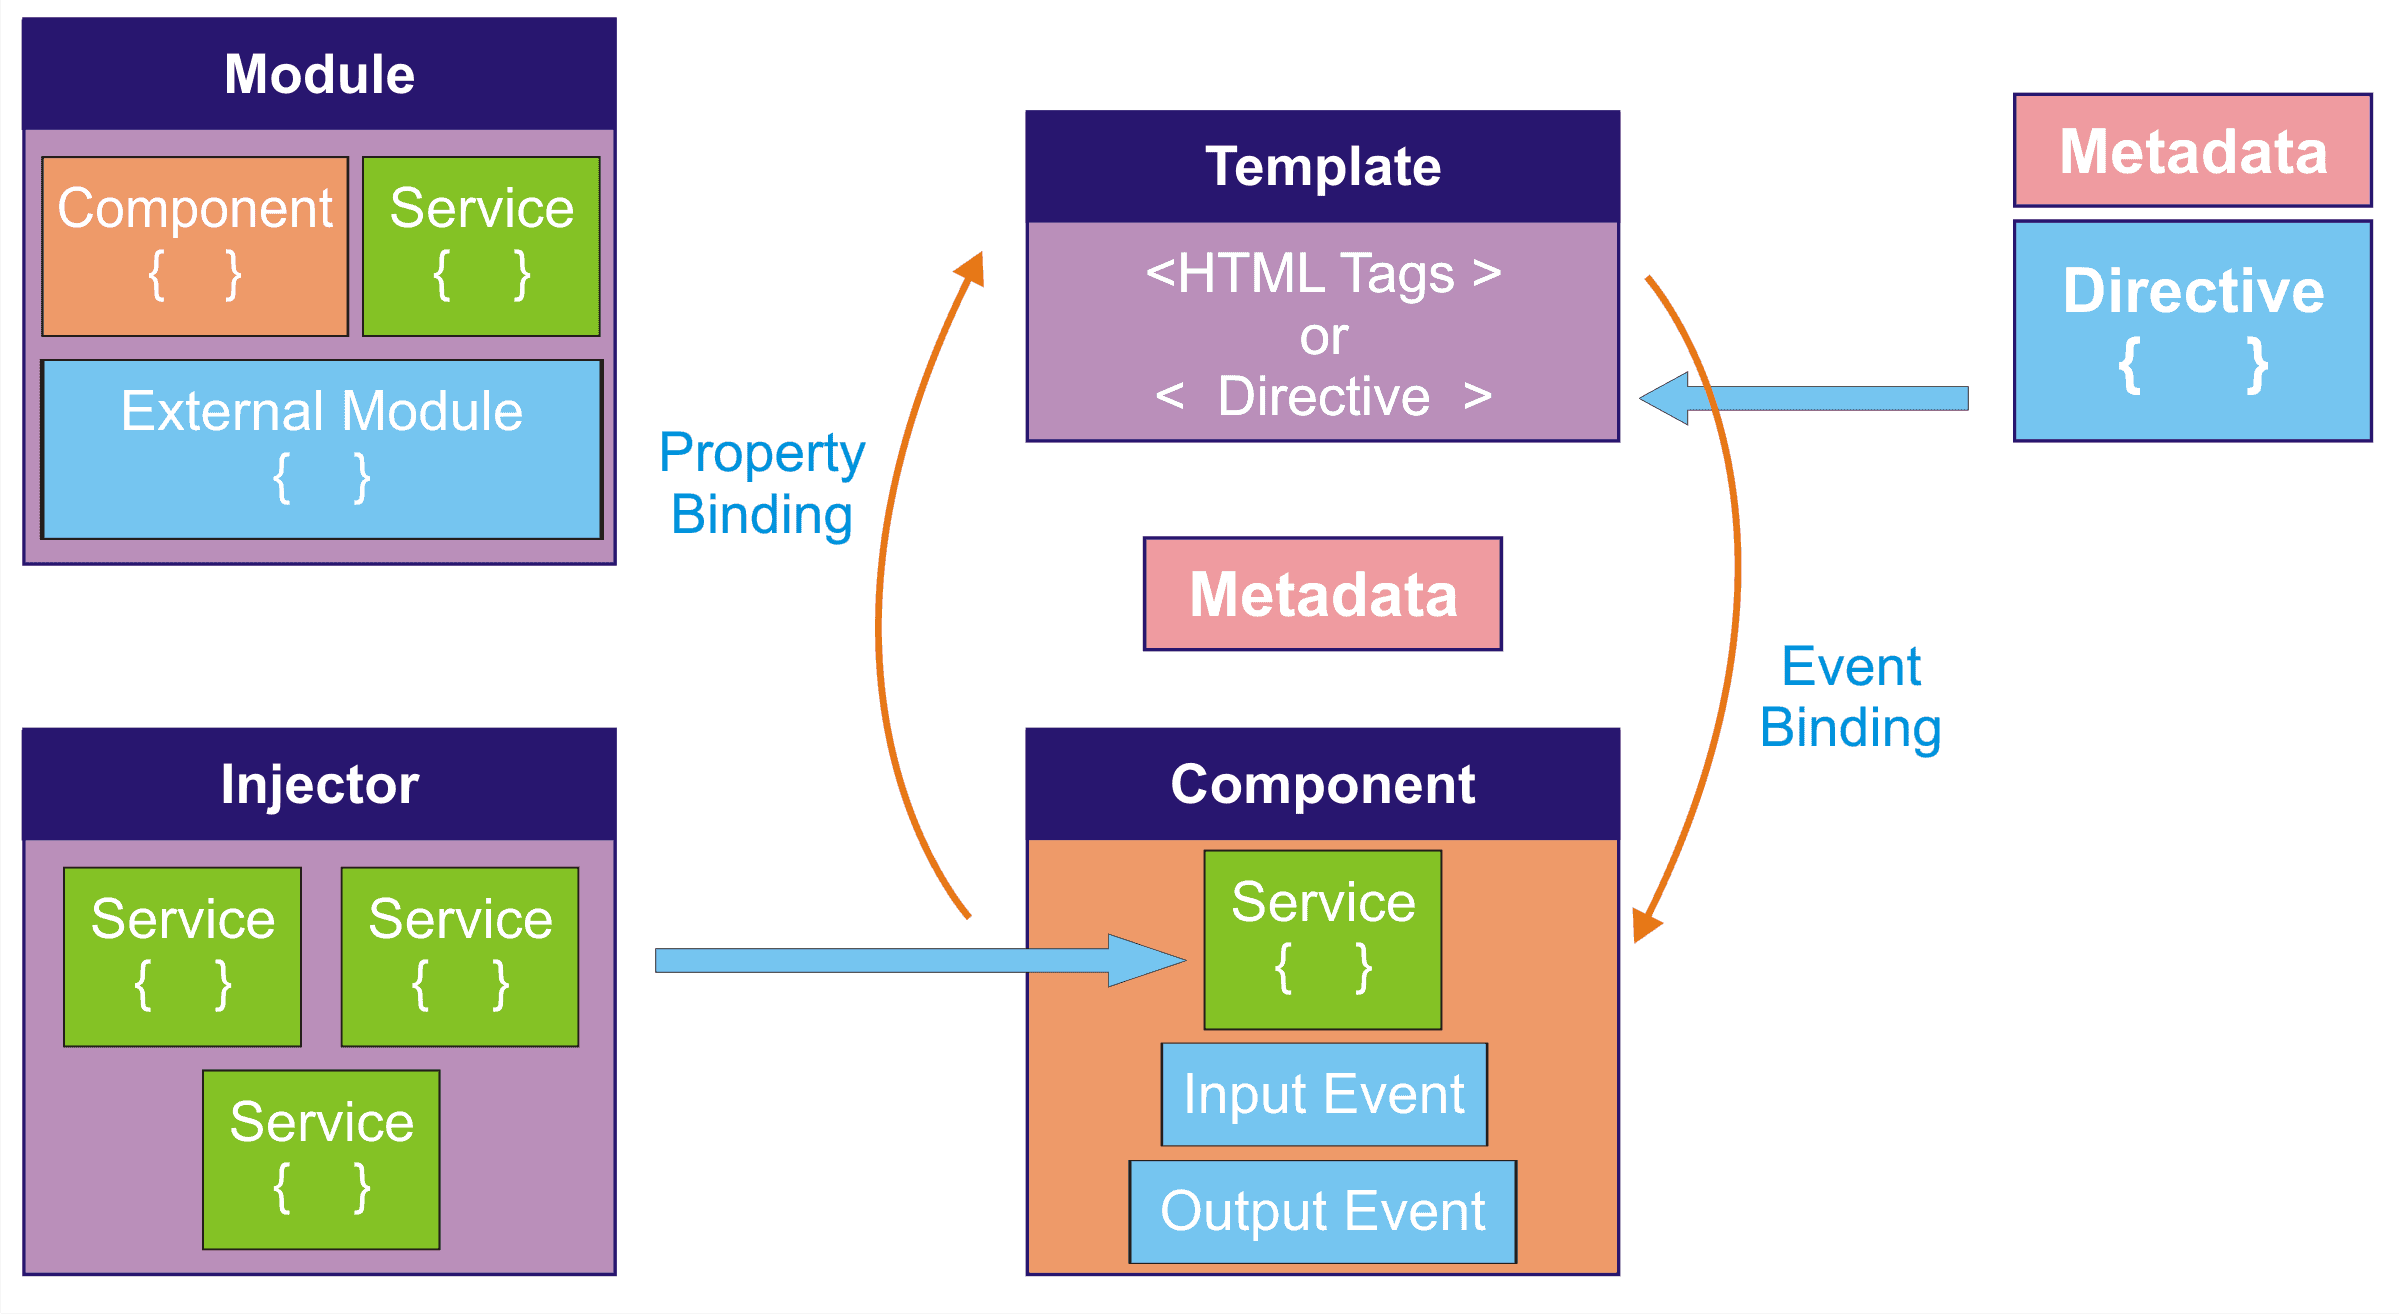
\includegraphics[width=0.8\textwidth]{Angular_Architecture.png}
	\caption{\url{https://www.ngdevelop.tech/wp-content/uploads/2017/12/Angular_Architecture.png}}
\end{figure}

\section{Spring Boot}
\begin{figure}[H]
	\centering
	
\includegraphics[width=0.3\textwidth, left]{Spring-boot-logo.jpg}
%	\caption{\url{https://dev.to/maddy/spring-boot-architecture-547i}}
\end{figure}

\textbf{Spring Boot} este un micro-framework open-source folosit pentru a crea aplicații Spring cu microservicii. Spre deosebire de alte framework-uri de Java, acesta oferă configurări XML flexibile, 
procesare în loturi puternică, tranzacții cu baza de date și o varietate de instrumente de dezvoltare.

\subsection{Scurt istoric}
Framework-ul \textit{Spring} a fost creat în 2004 pentru a simplifica dezvoltarea programelor pe partea de server. În aprilie 2014 a fost lansat Spring boot 1.0.0 în urma unor cereri din partea programatarilor de a configura serviciile de web container într-un container spring din metoda principală. În decembrie 2016 a fost lansat Spring Boot 1.3 ulterior trecerii framework-ului Spring de la versiunea 4.1 la 4.2 și includea sprinjin pentru fisiere JAR complet executabile, noi utilitare spring-boot-dev și auto-configurare pentru tehnologii de caching. 

\subsection{Motivație}
Spring Boot este bazat pe Java, unul dintre cele mai populare limbaje de programare. Framework-ul are o comunitate vastă de utilizatori cu diverse materiale și cursuri.

\begin{figure}[H]
	\centering
	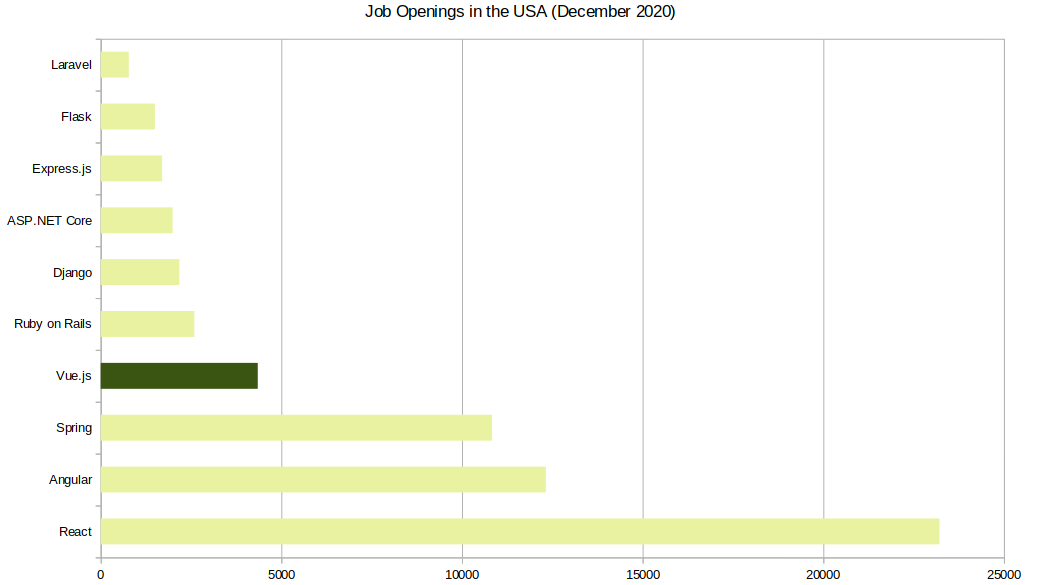
\includegraphics[width=0.8\textwidth]{Spring-ranking.png}
	\caption{\url{https://miro.medium.com/max/1400/1*Y6A_rS5IdRDUG4KRIFP_fA.png}}
\end{figure}

Avantajele prinicipale sunt după cum urmează. Spring Boot este \textit{multi-threaded}, util pentru operații repetitive și de durată. Facilitează crearea și testarea aplicațiilor Java oferind un setup default pentru unit și integration testing. Există de asemenea posibilitatea de a integra Spring Boot cu ecosistemul Spring ce include Spring Data, Spring Security, Spring ORM și Spring JDBC într-un mod simplificat.

\subsection{Particularități}
Principala particularitate a Spring Boot o reprezintă adnotările (\textit{Spring Boot annotations}) utilizate în auto configurare.
De exemplu, \textbf{@SpringBootApplication} marchează metoda principală a aplicației și este obligatorie.
\textbf{@EnableAutoConfiguration} oferă oricărei clase pe care o marchează cu opțiunea de Automatic Configuration.
\textbf{@ComponentScan} scanează la inițializare toate declarările de \textit{beans} și pachete.

Un alt detaliu este utilizarea \textit{Spring Starter Dependencies} ce facilitează gestionarea dependențelor unei aplicații în continuă dezvoltare.

\textit{Spring Boot Actuator} oferă utilitare de producție aplicației. Actuator este utilizat în mare parte pentru a obține informații de funcționare despre o aplicație în rulare (metrice, info, dump, env, etc.), cu ajutorul HTTp endpoints și JMX beans.
Ultima versiune, Spring Boot 2.x Actuator, suportă și modele CRUD.

\section{Cloud Firestore}
\begin{figure}[H]
	\centering
	
\includegraphics[width=0.3\textwidth, left]{Cloud-Firestore.png}
\end{figure}

\textit{Cloud Firestore} este un serviciu oferit de Firebase și este o bază de date în cloud, NoSQL, pentru a reține și sincroniza date între dispozitive folosind \textit{listeners} în timp real. Firestore oferă de altfel și suport pentru o integrare facilă cu serviciile Google Cloud.

\subsection{Particularități}
Fiind un model NoSQL, Firestore reține datele sub formă de \textit{documente} ce conțin câmpuri mapate la valori. Documentele formează la rândul lor diferite \textit{colecții}, containere folosite pentru organizarea datelor și crearea ușoară a cererilor (queries). Documentele pot reprezenta un număr mare de tipuri de date, de la string-uri până la tipuri complexe precum anumite obiecte. De asemenea, orice instanță, document, are posibilitatea să aibă subcolecții. Spre exemplu, în cazul de față, orice student ar putea avea drept subcolecție o listă de profesori reprezentând preferințele sale.

\subsection{Avantaje}
Cererile în cazul Cloud Firestore pentru crearea și primirea de date sunt expresive, flexibile și eficiente. Datele pot fi primite ușor sub forme de documente, iar posibilitatea de creare a subcolecțiilor ajută după caz la evitarea operațiilor costisitoare de join.

De asemenea, există opțiuni de sortare, filtrare și paginare a datelor primite.

Un avantaj important este reprezentat de \textit{realtime listeners} ce permit obținerea numai a informațiilor nou apărute, fără a extrage întreaga colecție de fiecare dată.

\subsection{Aplicabilitate}
Cloud Firestore are rolul în cazul acestei aplicații în principal de a reține participanții la procesul de repartizare, adică utilizatorii reprezentați de studenți și profesori, sub formă de documente. Fiecare document are o subcolecție de obiecte corespunzătoare reprezentând preferințele sale. Este de menționat că această subcolecție este sortată, fiind absolut necesară cunoașterea ierarhiei de opțiuni. Pe lânga preferințe, utilizatorii au și câmpuri specifice unei astfel de aplicații web, precum \textit{username}, \textit{email}, date administrative.

\section{Algoritmica}
\subsection{Problema stable matching (SMP)}
Problema constă în găsirea unei potriviri stabile (stable match) între două mulțimi de aceași dimensiune de elemente, luând în considerare o ierarhie a preferințelor. Astfel, o soluție este o bijecție între elementele primei mulțimi și cele din cea de a doua. O potrivire nu este stabilă dacă:

\begin{enumerate}
	\item Există un element $\alpha$ în mulțimea întâi care preferă un anumit element $\beta$ din cea de a doua mulțime în detrimentul unui element din a doua mulțime deja cuplat.
	\item $\beta$ preferă $\alpha$ în detrimentul elementului cu care $\beta$ deja este cuplat.
\end{enumerate}

Cea mai întâlnită formă a problemei este \textit{stable marriage problem}. Fie \textit{n} bărbați și \textit{n} femei, fiecare persoană având o ierarhizare a tuturor membrilor de gen opus în funcție de preferințe. 

Prima soluție a fost prezentată în 1962 de către David Gale și Lloyd Shapley care au demonstrat că pentru orice număr de participanți, există o soluție pentru a face toate cuplurile stabile.

\subsection{Algoritmul Gale-Shapley}
Algoritmul implică un număr de iterații. În prima iterație, fiecare element din prima mulțime A încearcă cuplarea cu prima sa obțiune din mulțimea B. Elementele din B sunt cuplate inițial cu elementul pretendent pe care îl preferă cel mai mult.

În iterațiile ulterioare, fiecare element din A necuplat încă încearcă să se cupleze cu următoarea opțiune din preferințele (necuplată sau nu). Elementele din B pot schimba partenerul curent cu cel propus în cazul în care este deja cuplată dacă îl preferă pe cel din urmă.

Procesul se repetă până când există o bijecție între cele două mulțimi.

\subsection{Instanța problemei prezente}
În cazul problemei distribuirii studenților la profesorii coordonatori de licență, fiecare student primind implicit o temă unică de licență, există atât asemănări cu \textit{SMP} (Stable Marriage Problem), cât și o serie de deosebiri particulare care necesită o adaptare a algoritmului de rezolvare.

\textbf{Asemănări}

Există două mulțimi ce trebuie cuplate într-un mod stabil. Cuplajul este realizat tinând cont și în această instanță de o serie de preferințe. Ambele tipuri de participanți au o ierarhizare a preferințelor sale. Din punct de vedere al temelor de licență, cel mai probabil există o relație de bijecție între studenți și tematicile primite sau propuse și acceptate.

\textbf{Deosebiri}

O primă deosebire observată este că mulțimile nu au un număr egal de elemente. În mod natural, mulțimea studenților este semnificativ mai mare decât cea a profesorilor.

În al doilea rând, relația dintre cele două mulțimi nu este de bijecție, ci mai degrabă una injectivă. Fiecare student trebuie să aibă la finalul procesului de repartizare atribuit un profesor coordonator de licență. Cu alte cuvinte,

\[\forall \: stud,\: unde\: stud \in Studs,\: \exists \: prof \in Profs,\] 
\[BTD(stud)=prof\]

unde \textit{BTD} = Bachelor Thesis Distributor, funcție ce repartizează fiecare student unui profesor, \textit{Studs} = mulțimea studenților, \textit{Profs} = mulțimea profesorilor.

În consecință, este inevitabil ca un profesor să aibă sub coordonare mai mulți studenți, o altă particularitate fiind însă că un profesor are o limită prestabilite de astfel de studenți.

La finalul procesului de repartizare, studenții care nu au o preferință sunt repartizați aleatoriu sau după un anumit criteriu arbitrar profesorilor care mai au locuri libere.
